%\documentclass[t,handout]{beamer}
\documentclass{beamer}


\usepackage[utf8]{inputenc}
\usepackage[portuguese]{babel}
\usepackage[tight]{subfigure}
\usepackage{graphicx}
\usepackage{color}
\usepackage{url}
% \usepackage{listings}
%\usepackage[alf]{abntcite}

%Pacote de listagem de c�digo
\usepackage{listings}
\lstset{numbers=left, stepnumber=1, firstnumber=1,
numberstyle=\tiny, extendedchars=true, breaklines=true, frame=tb,
basicstyle=\footnotesize, stringstyle=\ttfamily,
showstringspaces=false }


%\usetheme{Frankfurt} %LEGAL     !!!
% \usetheme{Madrid}     %LEGAL/L%IMPO/COM CAIXA     (sem barra de desenvolvimento)

% \usetheme{Antibes} %NAO
%\usetheme{Berlin} %PODE SER...     (BARRA DE DESENVOLVIMANTO)
% \usetheme{Berkeley}     %FEIO
% \usetheme{Boadilla} %TUDO BRANCO...
% \usetheme{Copenhagen}     %NAO
% \usetheme{Darmstadt} %LEGAL!     !!!
 \usetheme{Dresden}     %LEGAL/LIMPO/SEM CAIXA     (sem caixa fica ruim...)

% \usetheme{Goettingen}     %FEIO DEMAIS!
%\usetheme{Ilmenau} %LEGAL (forte candidato)
% \usetheme{JuanLesPins} %BACANA
% \usetheme{Luebeck}     %FEIO

% \usetheme{Malmoe}     %FEIO
% \usetheme{Warsaw} %NAO...
% \usetheme{Seattle}
% \usetheme{CambridgeUS}
% \usetheme{Singapore}

% \usecolortheme[RGB={130,35,150}]{structure}
% \usecolortheme[RGB={33,33,94}]{structure}
\usecolortheme[RGB={134,153,188}]{structure}
\setbeamertemplate{footline}[frame number]
\setbeamertemplate{navigation symbols}{}

%Hide subsections on teable of contents
%\hypersetup{bookmarksopen=true,bookmarksopenlevel=4}
%\setcounter{tocdepth}{2}



\author[L. Medeiros]{Aluno: Leonardo Melo de Medeiros}
%\date{\today}
\date{03/06/2016}
\institute[]{Orientador: Leandro Dias da Silva\\
						 Orientador: Hyggo Oliveira de Almeida \\ 
						 Universidade Federal de Campina Grande - UFCG}
\title{Uma Abordagem de Monitoramento dos Sinais Motores da Doença de Parkinson Baseada em Jogos Eletrônicos}
%\logo{
\includegraphics[width=0.2\linewidth]{img/logo.png}}
\subtitle{Defesa de Tese}

\begin{document}

\begin{frame}
  \titlepage
\end{frame}

% \section{Roteiro}
% \AtBeginSection[]
{\frame{
\frametitle{Roteiro}
%\tableofcontents
\tableofcontents[hideallsubsections]
}
}





\section{Introdução}
\subsection{Motivação}

\begin{frame}{Sistemas de Monitoramento da Saúde (SMS)}  
  \begin{block}{}
  Atualmente, os Sistemas de Monitoramento da Saúde (SMS) permitem ao médico:
  \begin{itemize}
   \item Tratar preventivamente e pró-ativamente o estado de saúde~\cite{healthmonitoring2013}
   \item Reabilitar o paciente~\cite{sacbespoke2014}
   \item Melhorar a qualidade de vida~\cite{sacsvmhms2014}
  \end{itemize} 
  \end{block} 
\end{frame}


\begin{frame}{Principais Desafios dos (SMS)}
  \begin{block}{}
  \center
      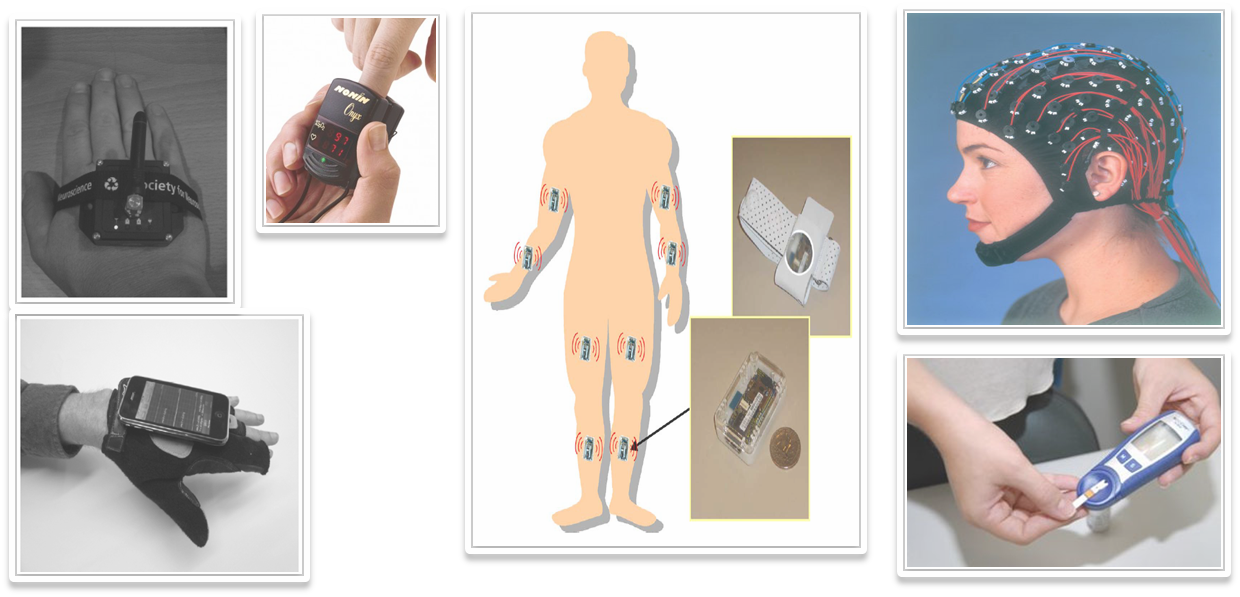
\includegraphics[height=1.8 in]{img/sismonsaude.png}
  \end{block}
  \begin{block}{}  
  A concepção de um sistema não invasivo de monitoramento é um grande desafio~\cite{alemdar2015}
  \end{block}
\end{frame}





\begin{frame}{Estratégias de Monitoramento da Saúde}
  \begin{block}{}
      \center 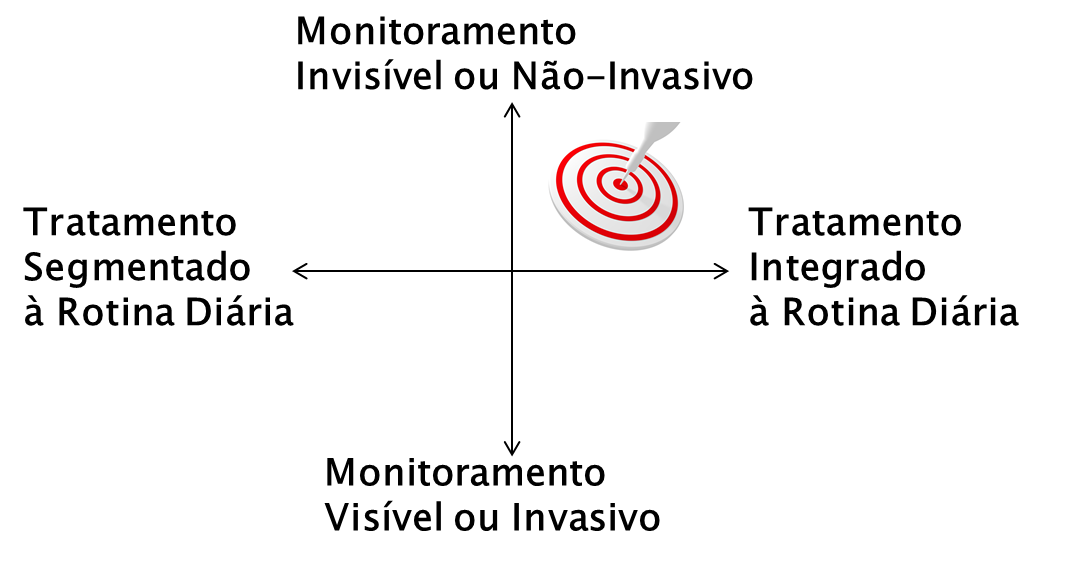
\includegraphics[height=2.2 in]{img/estrategmonitorament.png}
  \end{block}
%   \begin{block}{}
% As tecnologias de monitoramento para serem aceitas precisam preservar a privacidade do usuário e integrar-se à sua rotina diária~\cite{alemdar2015}.
%   \end{block}
\end{frame}


\begin{frame}{SMS Motores}  
  \begin{block}{}  
  Atualmente, os SMS motores permitem:  
    \begin{itemize}
    \item Quantificar as habilidades motoras dos usuários~\cite{manumeterjbhi2014,patel_monitoring_2009}
    \item Analisar a marcha dos usuários~\cite{robotgait2014}
    \item Identificar sinais de bradicinesia (lentidão dos movimentos) presente no Parkinson~\cite{ambulatoryparkinson2010}
    \end{itemize}   
  \end{block}   
\end{frame}

\begin{frame}{Abordagem Proposta}
  \begin{block}{}
      \center 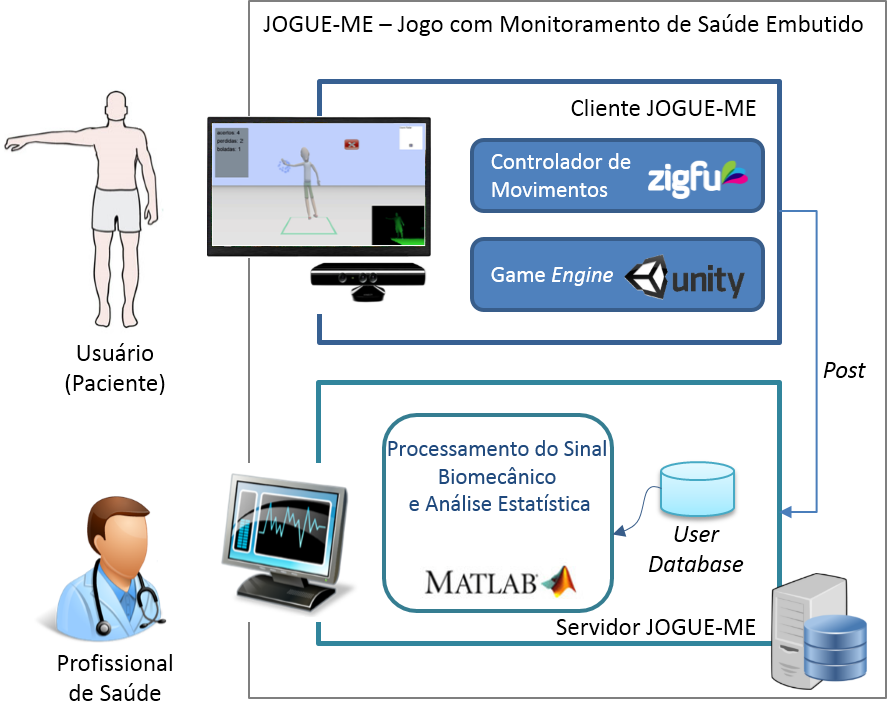
\includegraphics[height=1.8 in]{img/visaosistema.png}
  \end{block}
  \begin{block}{}
Nesta tese, propus monitorar a saúde de uma forma não invasiva usando jogos eletrônicos
  \end{block}
\end{frame}


\begin{frame}{Cenário de Uso}
   \begin{block}{}
      Como possível cenário de uso para a pesquisa, supondo que:
      \begin{itemize}
       \item Um paciente faz uso do cliente JOGUE-ME no \textbf{conforto de seus lar} e, consequentemente, fornece os sinais motores em diferentes momentos do dia
       \item Logo, esses sinais motores são \textbf{quantificados e enviados} para o servidor JOGUE-ME
       \item O servidor \textbf{JOGUE-ME analisa os sinais e identifica a ocorrência} do sintomas motor
       \item Então, o \textbf{médico acessa a informação} sobre a saúde motora e \textbf{consegue melhor gerenciar a saúde} de seus pacientes 
      \end{itemize}
  \end{block}
\end{frame}


\subsection{Jogos Para Saúde}
\begin{frame}{Jogos Aplicados à Saúde}
	\begin{block}{}	
	Nos últimos anos, houve o surgimento de jogos para apoiar a prática de atividade física. Como por exemplo:
	
	\begin{itemize}
	    \item Melhoria da saúde do idoso com: visando a reabilitação motora~\cite{sacbespoke2014}
	    \item Jogo com sensor háptico para quantificar a habilidade motora do paciente com Parkinson~\cite{atkinson2010}
	    \item Jogo para o monitoramento dos sinais vitais(Batimento cardíaco)~\cite{Sinclair:2009:UVB:1515604.1515617}
	\end{itemize}
	\end{block}
\end{frame}


\begin{frame}{Motivação para uso de jogos para monitoramento dos dados motores}
	\begin{block}{}
	\begin{itemize}
	    \item Percentual expressivo de adultos e idosos que usam jogos em sua rotina diária (27\% acima dos 50 anos~\cite{esa2015})
	    \item As tecnologias de sensores de movimento estão presentes nos jogos eletrônicos
	    \item Reprodução de movimentos específicos em um ambiente lúdico e longe do tratamento de saúde
	\end{itemize}
	\end{block}
	
% 	\begin{alertblock}{}
% 	Monitorar os sinais permite um melhor gerenciamento da doença e, por consequência, uma melhora na qualidade de vida
% 	\end{alertblock}
\end{frame}


\begin{frame}{Objetivo Principal}
  \begin{block}{}
  Conceber um SMS embutido num jogo eletrônico para \textbf{motivar e abstrair o monitoramento dos sinais motores de uma maneira não invasiva e integrada à rotina diária}
  \end{block}
\end{frame}


\begin{frame}{Etapas do Trabalho}
	\begin{block}{}
	  A da metodologia deste trabalho consistiu de três etapas sequenciais:
		  \begin{description}
		  \item[ETAPA 1] Quais os benefícios de acompanhar os sinais motores do paciente diariamente, do ponto de vista do profissional da saúde?
		  \item[ETAPA 2] Como melhor adquirir e quantificar sinais motores utilizando sensores de movimento para monitorar os sinais do Parkinson?
		  \item[ETAPA 3] Na perspectiva dos usuários, a abordagem de quantificar os sinais motores é considerada não-invasiva e aplicável à rotina diária?
		  \end{description}
	\end{block}
\end{frame}

\section{Estudo de Caso}
\subsection{Parkinson}
\begin{frame}{Estudo de Caso}
  \begin{block}{}
   Como estudo de caso, foi utilizada a Doença de Parkinson (Parkinson) por ser uma doença debilitante, progressiva e que possui uma grande \textbf{flutuabilidade dos sintomas com o tratamento medicamentoso}
   %\begin{itemize}
    %\item Comum em idosos
    %\item Existem casos precoces em indivíduos antes dos 40 anos
    %\item 
   %\end{itemize}
  \end{block}
\end{frame}


\begin{frame}{Parkinson}
  \begin{block}{}
    O Parkinson é uma afecção do sistema nervoso central, que afeta aproximadamente a 2\% dos idosos e não possui ainda diagnóstico estabelecido. 
		
		O diagnóstico é dado pelo neurologista na análise clínica dos sinais cardinais de \textbf{rigidez, bradicinesia, tremor e instabilidade postural}~\cite{jankovic2008} e a resposta positiva ao tratamento medicamentoso~\cite{protpar010}
%   \begin{block}{Termos: Tremor de Repouso e Bradicinesia}<3->
%       \begin{itemize}
%        \item \textbf{Tremor de Repouso:} sintoma mais frequente e perceptível;
%        \item \textbf{Bradicinesia:} lentidão na execução do movimento;
%       \end{itemize}
   \end{block}
\end{frame}


\begin{frame}{Parkinson}
  \begin{block}{Sintoma de bradicinesia}
      \begin{itemize}
	\item Enquanto que o tremor é o sintoma motor mais visível do Parkinson, a bradicinesia é o mais incapacitante
	%\item A bradicinesia consiste numa lentidão do movimento voluntário e num comprometimento de todos os movimentos associados a ele.
	\item A bradicinesia é acompanhada de: rigidez dos músculos, assimetria dos movimentos e dificuldade nos movimentos
	\end{itemize}
  \end{block}
\end{frame}
  

\begin{frame}{Estágios da Doença}
  \begin{block}{Escala Unificada de Avaliação da Doença de Parkinson (UPDRS)}
    %A escala UPDRS avalia tanto o nível de estrutura e função corporal quanto o nível das atividades.
      A escala contém itens referentes a:
	\begin{itemize}
	 \item Mental, comportamento e humor
	 \item Atividades da vida diária
	 \item Exame motor
	 \item Complicações no tratamento
	\end{itemize}
 \end{block}
\end{frame}

\begin{frame}{Escala (UPDRS)} 
%    \begin{block}{}
      \center 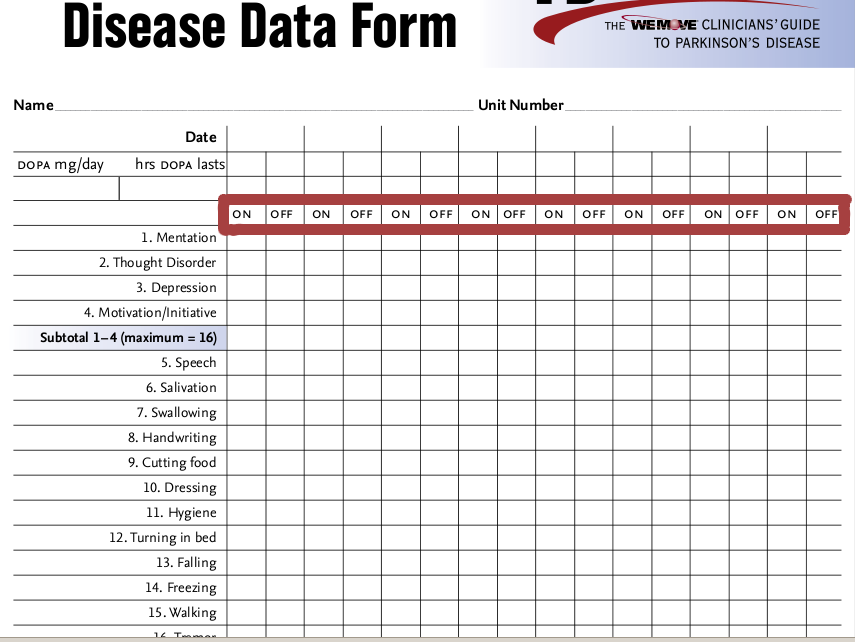
\includegraphics[height=2.0 in]{img/updr1-sel.png}
     \begin{itemize}
	\item Avaliação dos sintomas de maneira subjetiva e esporádica
	\item Flutuação dos sintomas (fenômeno \textit{on/off})
     \end{itemize}
%    \end{block}

\end{frame}

% \begin{frame}{Escala (UPDRS)} 
%     \begin{block}{Impacto nas Atividades Diárias}
%       \center 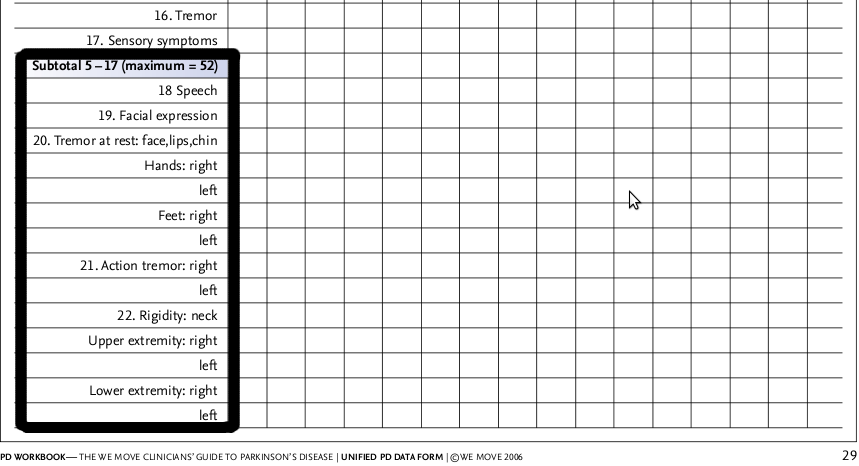
\includegraphics[height=2.0 in]{img/updr2-sel.png}'
%     \end{block}
% \end{frame}


\subsection{Entrevista}
\begin{frame}
  \begin{block}{ETAPA 1}
   Quais os benefícios de acompanhar os sinais motores do paciente diariamente, do ponto de vista do profissional da saúde?
  \end{block}
\end{frame}

\begin{frame}{Entrevista Semi-Estruturada com Profissionais de Saúde} 
    \begin{block}{Objetivo da Pesquisa}
    O objetivo da entrevista semiestruturada foi entender como é feito o acompanhamento do paciente com sintomatologia do Parkinson, juntamente aos profissionais de saúde
    \end{block}
		\begin{block}{Participantes}
			\begin{table}[h]
			%\caption{Perfil dos Participantes}
			%\label{table:perfil_analise_participantes}
			\begin{tabular}{|l|l|c|c|}
			\hline
			\textbf{LEGENDA} & \textbf{PROFISSÃO}             & \multicolumn{1}{|l|}{\textbf{EXPERIÊNCIA (ANOS)}} \\ \hline
			FIS\_01          & Fisioterapeuta & 10                                                \\ \hline
			FIS\_02          & Fisioterapeuta    & 10                                                \\ \hline
			NEU\_01          & Neurologista            & 15                                                \\ \hline
			NEU\_02          & Neurologista            & 30                                                \\ \hline
			\end{tabular}
			\end{table}
    \end{block}
\end{frame} 


\begin{frame}{Análise dos fragmentos da entrevista} 
    \begin{block}{}			
			Um ponto de convergência entre os profissionais entrevistados é a importância de monitorar a velocidade angular dos pacientes.
		\end{block}
		
		\begin{block}{}
					Como pode ser analisado nesta citação de um dos neurologistas:
			\begin{quote}
				\textbf{[FRAGMENTO-14][NEU\_01]} 
					\emph{
						``É como eu falei, para mim seria melhor se capturássemos se ele está mais lento. Se através dessa amplitude, você conseguir por intermédio do computador identificar que ele está mais lento de um lado do que do outro, e conseguir visualizar a velocidade de um lado e do outro. Então, isso é interessante.''
			}
			\end{quote}			
    \end{block}
\end{frame} 






\begin{frame}{Resultado da Entrevista} 
    \begin{block}{}
			\begin{itemize}
				\item Identifiquei a importância de \textbf{monitorar a bradicinesia para acompanhar a evolução do Parkinson}
				\item Os profissionais de saúde informaram da importância de calcular:
					\begin{enumerate}
						\item amplitude dos movimentos de abdução e adução dos braços
						\item a velocidade angular desse movimento
					\end{enumerate}
			\end{itemize}
    \end{block}
\end{frame} 




\section{Abordagem JOGUE-ME}


\subsection{Apresentação}
\begin{frame}
  \begin{block}{ETAPA 2}
   Como melhor adquirir e quantificar sinais motores utilizando sensores de movimento para monitorar os sinais do Parkinson?
  \end{block}
\end{frame}

\begin{frame}{Abordagem JOGUE-ME}
    \begin{block}{}
    A abordagem \textbf{JOGUE-ME} faz uso de jogos eletrônicos como interface de aquisição de sinais, tornando os usuários mais motivados a fornecer seus dados motores
    \end{block}
    
    
    \begin{block}{}
    Este trabalho pretende usar um ambiente de jogo para a execução de movimentos específicos, com o propósito de quantificar os sinais motores dos usuários e, consequentemente, realizar o monitoramento
    \end{block}
\end{frame}

\begin{frame}{Visão Geral da Abordagem~\textit{JOGUE-ME}}
  \begin{block}{}
      \center 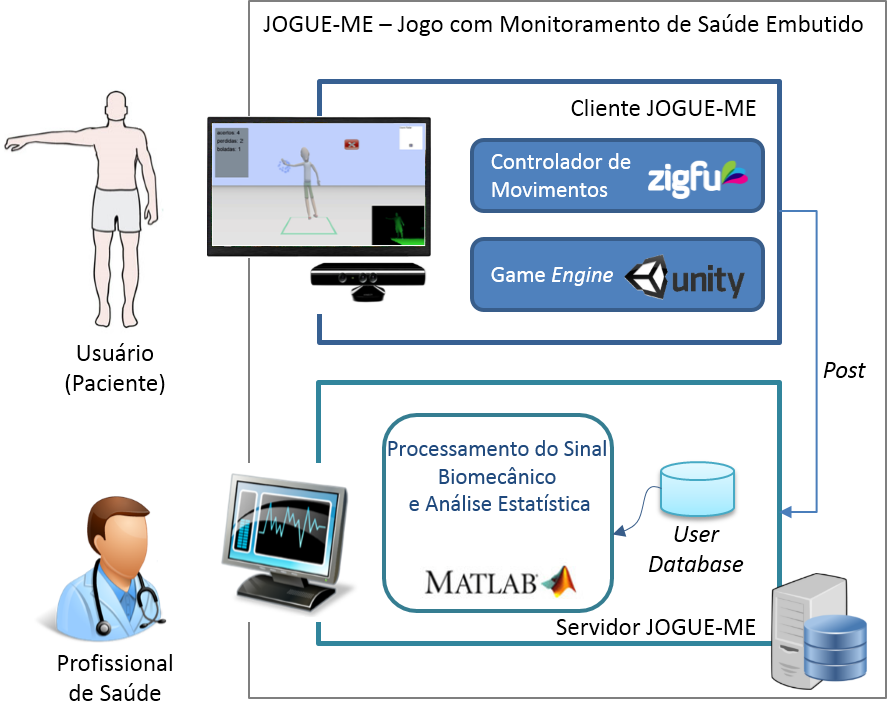
\includegraphics[height=2.2 in]{img/visaosistema.png}
  \end{block}
\end{frame}


\begin{frame}{JOGUE-ME - \textit{Jogo com Monitoramento de Saúde Embutido}}
	\begin{block}{}
		\begin{itemize}
			\item	\textbf{REQ-JOGUE-ME-01} - Pontuação e taxa de acerto
			\item	\textbf{REQ-JOGUE-ME-02} - Progresso e evolução do jogador e dos desafios
			\item	\textbf{REQ-JOGUE-ME-03} - Estado de fluxo
			\item	\textbf{REQ-JOGUE-ME-04} - Preocupação com integridade física do jogador
			\item	\textbf{REQ-JOGUE-ME-05} - Aquisição e armazenamento de sinais motores
			\item	\textbf{REQ-JOGUE-ME-06} - Mecanismo de identificação de sintomas motores
			\item	\textbf{REQ-JOGUE-ME-07} - Mecanismo de visualização
		\end{itemize}
	\end{block}
\end{frame}

\subsection{Processamento de Sinais}


\begin{frame}{Estudo Biomecânico da Cinemática Angular}
  \begin{block}{}
      \begin{itemize}
	 \item A cinemática angular permite examinar o movimento angular a partir de segmentos de um movimento, divididos em partes identificáveis que aumentam a compreensão do movimento humano  
	 \item Estudo das forças e momentos que resultam no movimento do corpo e seus segmentos
	 \item Processamento das grandezas cinemáticas considerando: 
	    \begin{enumerate}
	      \item tempo
	      \item ângulo
	      \item amplitude
	      \item velocidade angular
	    \end{enumerate}
       \end{itemize}
  \end{block}
\end{frame}


\begin{frame}{Sensor de Captura de Movimentos}
  \begin{block}{}
      \center 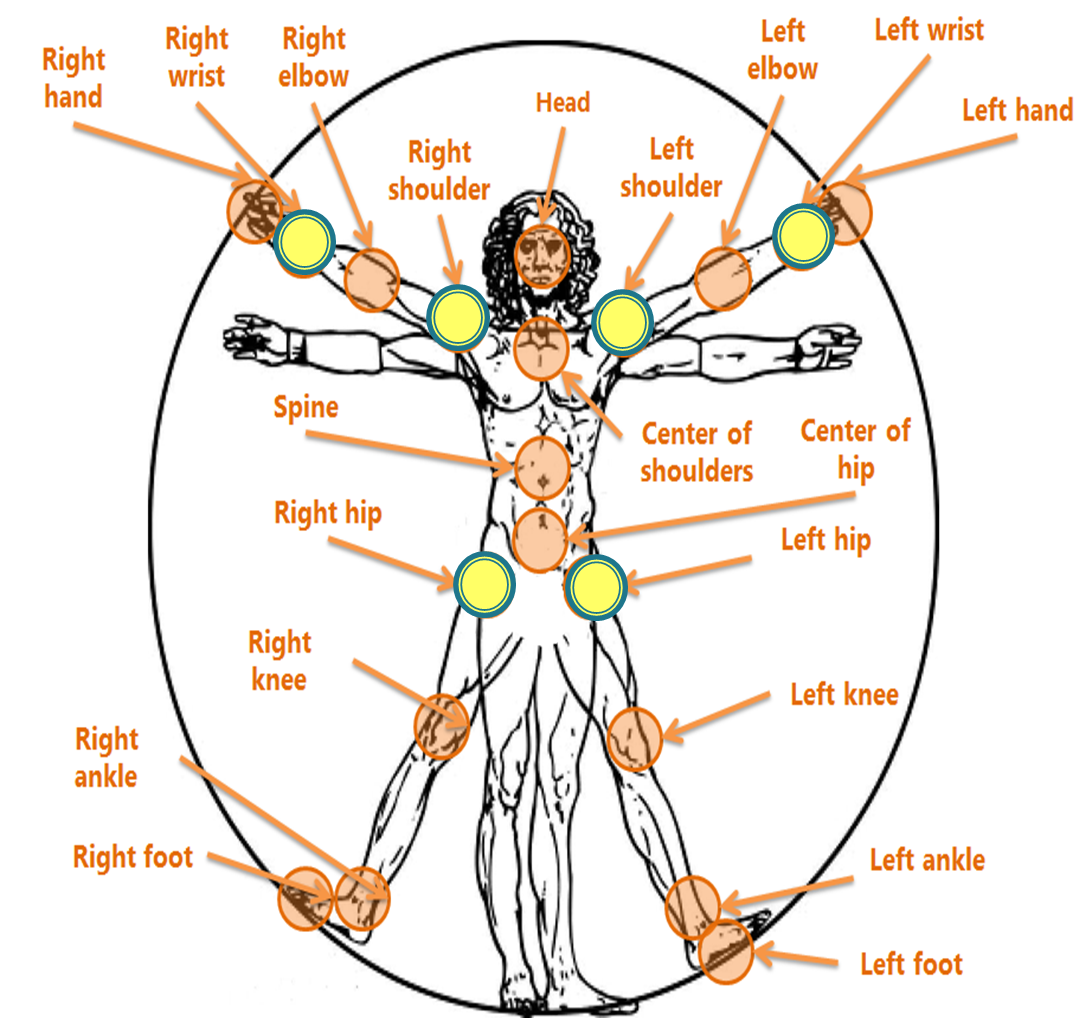
\includegraphics[height=2.5 in]{img/articulacoes-sel.png}
			%\caption{Modificações no Jogo ao Longo das Fases de Desenvolvimento~\cite{fullerton2008game}}
  \end{block}
\end{frame}

\begin{frame}{Movimento Angular}
  \begin{block}{Movimento de Abdução e Adução do Braço ~\cite{mcginnis2013biomechanics}}
      \center 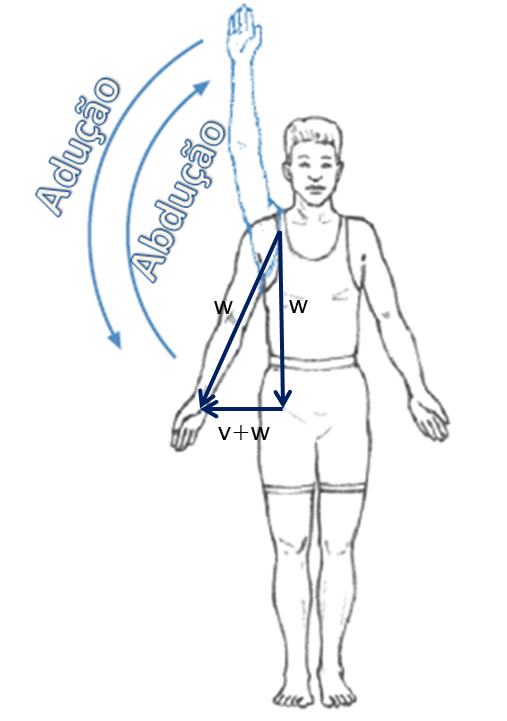
\includegraphics[width=4cm]{img/abducao-angulo.png}
  \end{block}
\end{frame}



\begin{frame}{Mecanismo de Identificação de Sintomas Motores}
      \center 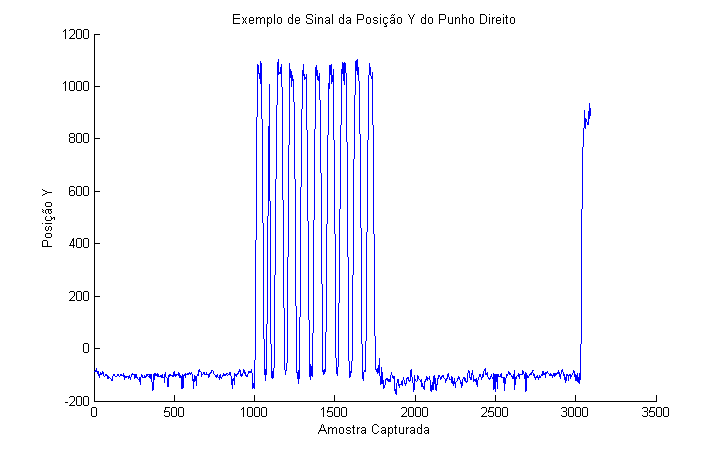
\includegraphics[height=2.8 in]{img/exsinalposicaoypunhodireito.png}
\end{frame}



\begin{frame}{Técnicas de Picos e Vales do Sinal}
  %\begin{block}
      \center 
      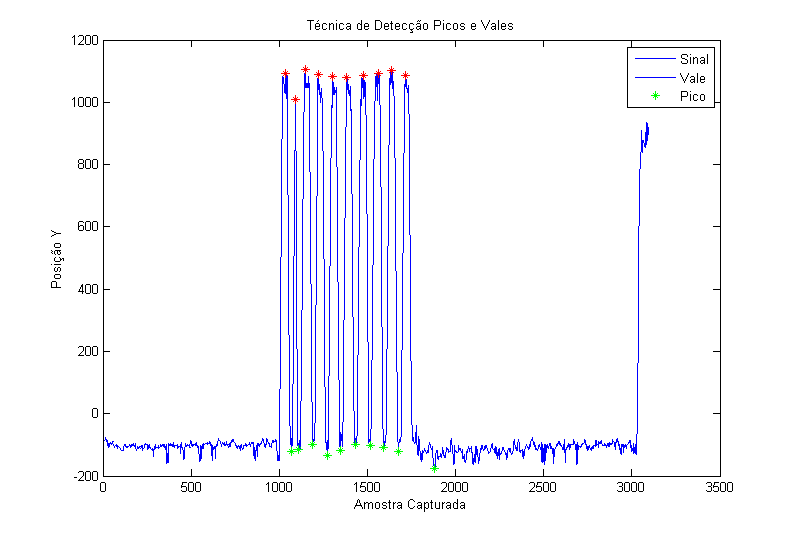
\includegraphics[height=2.8 in]{img/deteccaopicosvales.png}
  %\end{block}
\end{frame}



\begin{frame}{Velocidade Angular do Movimento de Abdução e Adução}
     %\begin{block}{}
      \center 
      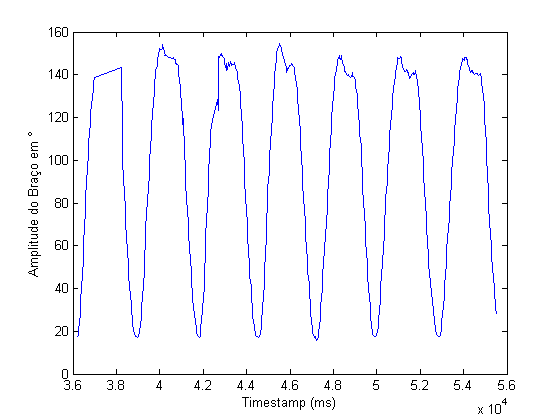
\includegraphics[height=2.8 in]{img/amplitude-braco.png}
			%\caption{Modificações no Jogo ao Longo das Fases de Desenvolvimento~\cite{fullerton2008game}}
     %\end{block}
\end{frame}

\begin{frame}{Filtragem de Dados: Remoção de Ciclos Incompletos}
   \begin{block}{}
   
   \begin{columns}[c]
     \begin{column}{0.5\linewidth}
				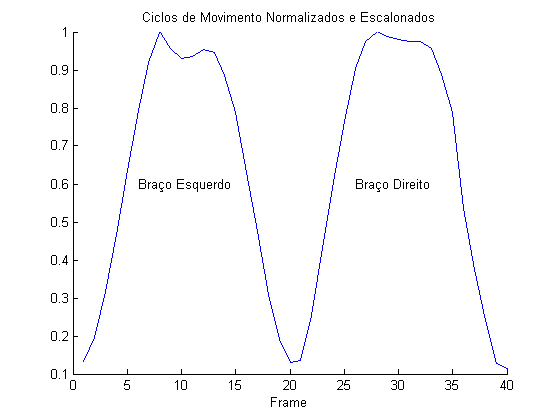
\includegraphics[width=5.5cm]{img/ciclonormalizadoescalonado.png}
     \end{column}

     \begin{column}{0.55\linewidth}
				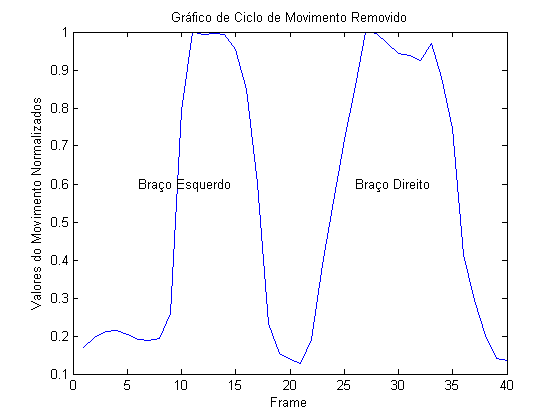
\includegraphics[width=5.5cm]{img/ciclomovimentoremovido.png}
    \end{column}
\end{columns}
\end{block}
\end{frame}

\begin{frame}{Visualização das Características do Movimento}
  \begin{block}{}
      \center 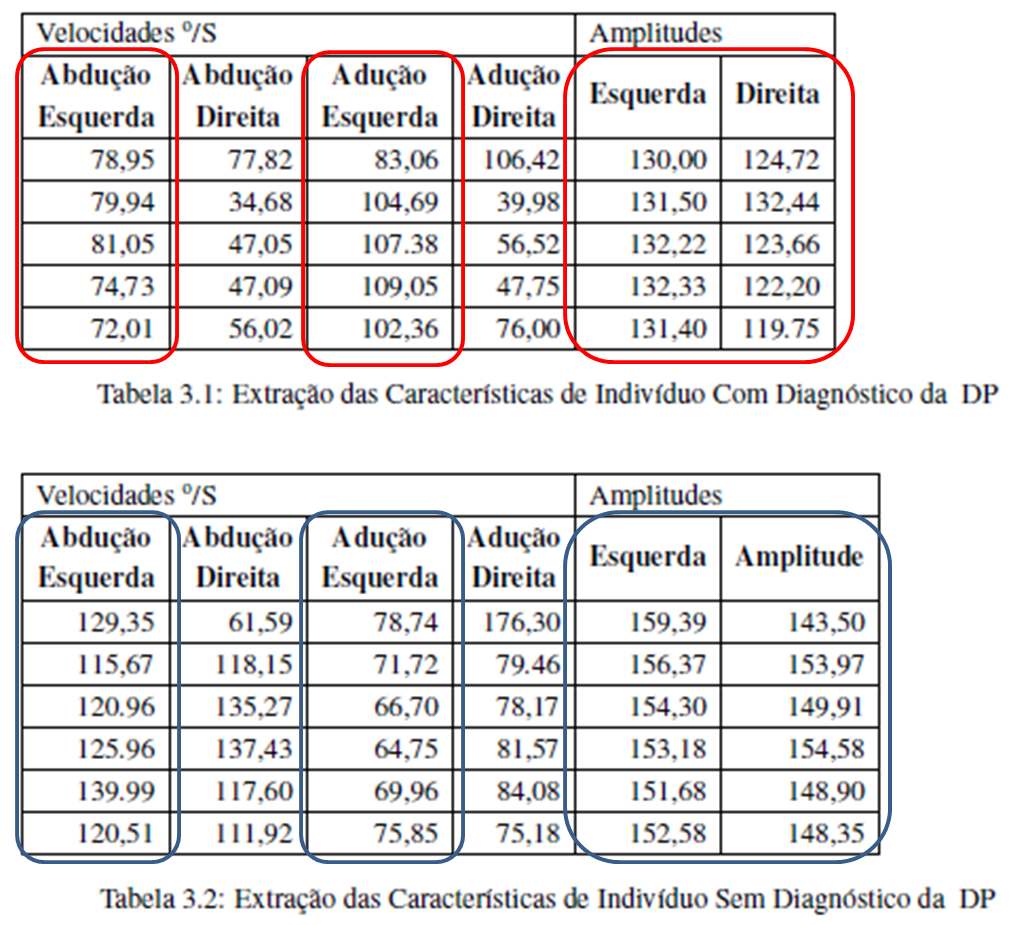
\includegraphics[height=2.2 in]{img/caracteristicas-tabela.png}
			%\caption{Modificações no Jogo ao Longo das Fases de Desenvolvimento~\cite{fullerton2008game}}
  \end{block}
\end{frame}

\subsection{Classificador de Dados}
\begin{frame}{Classificador de Dados}
\begin{block}{}
			Nesta tese, a Máquina de Vetor de Suporte (SVM) foi usada como método de aprendizagem supervisionada para problemas de classificação.
			
			A escolha da SVM deveu-se a sua elevada capacidade de \textbf{generalização} na previsão de dados não treinados, e na \textbf{robustez} em grandes dimensões de dados, por ex., \textbf{análise de sinais}.			
\end{block}
\end{frame}



\begin{frame}{Processamento dos Sinais Biomecânicos}
  
      \left 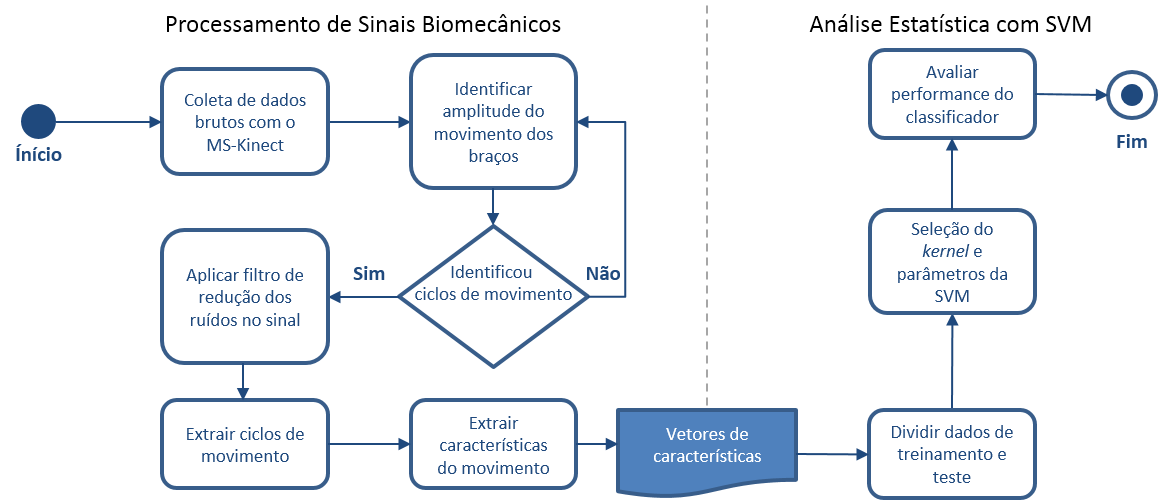
\includegraphics[height=1.9 in]{img/biomecprocessorh.png}
  
\end{frame}



% \begin{frame}{Visualização do Vetor Médio do Movimento de Abdução e Adução do Braço}
%       \center 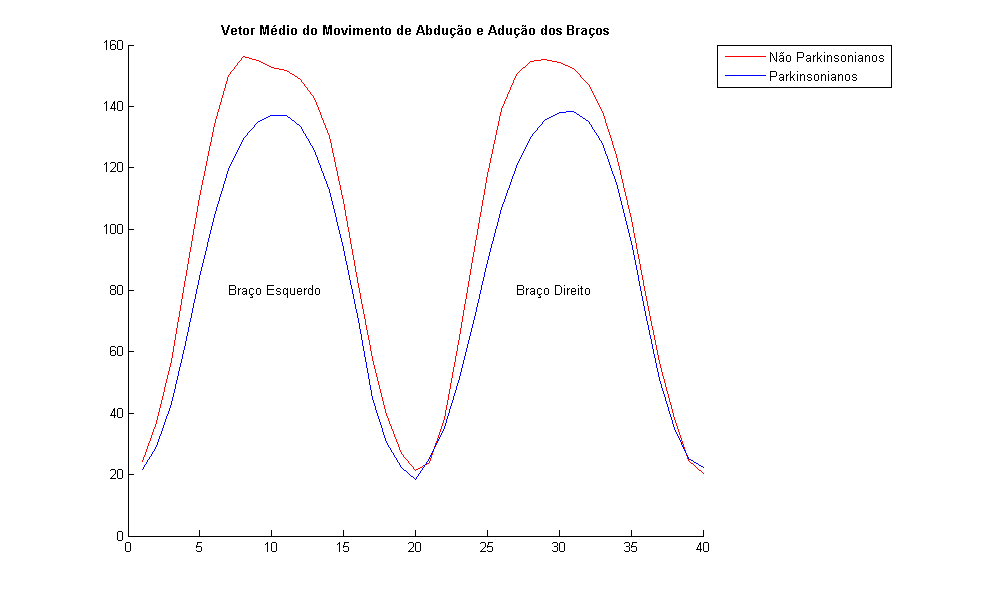
\includegraphics[height=2.6 in]{img/vetormedioaducao.png}
% \end{frame}

% \begin{frame}{Ciclos de Movimento de Abdução e Adução do Braço}
%       \center 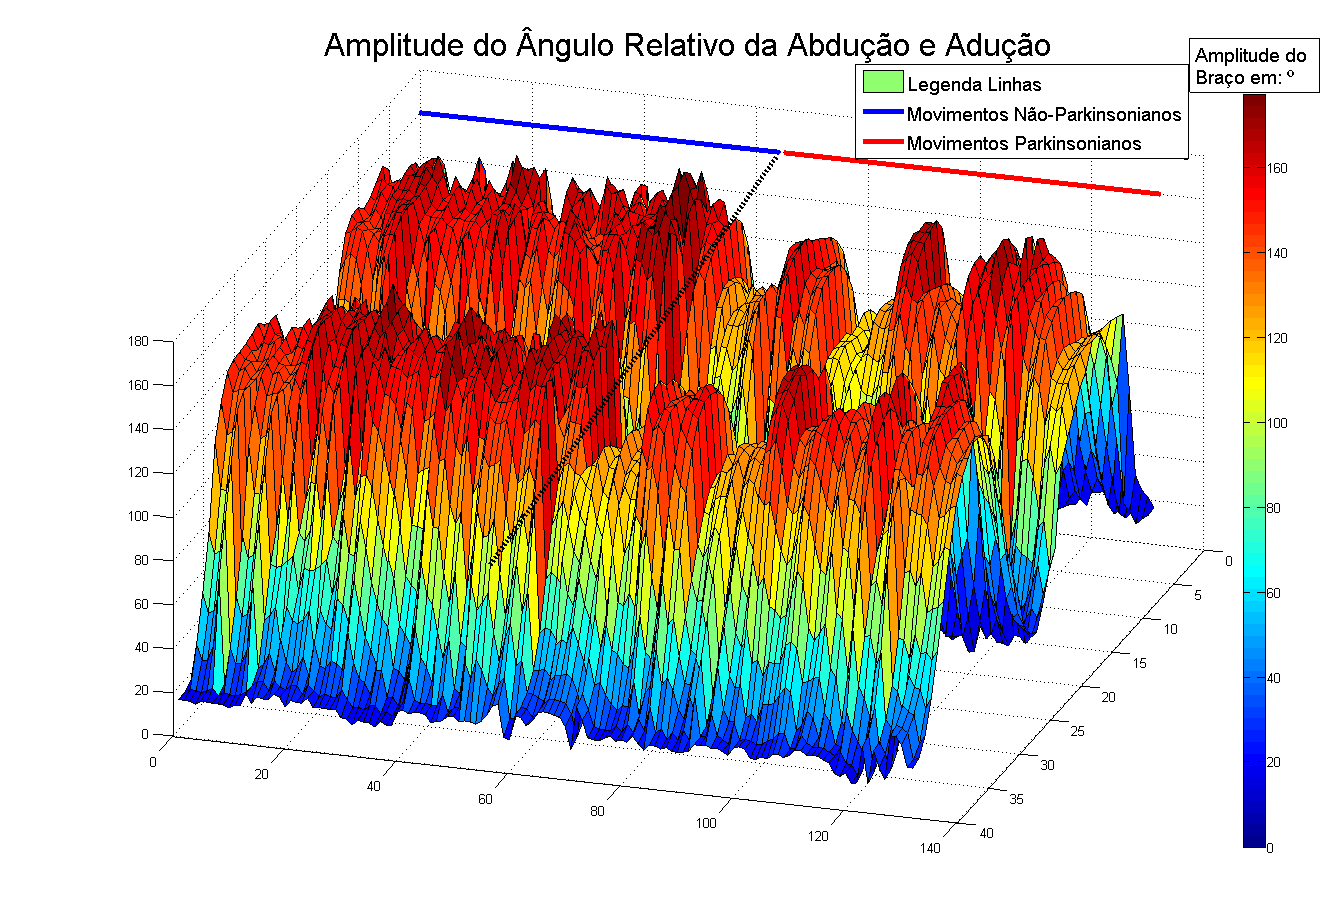
\includegraphics[height=3 in]{img/ciclosmovimentokinnect-2.png}
% \end{frame}


% \begin{frame}{Visualização das Características do Movimento}
%   \begin{block}{}
%       \center 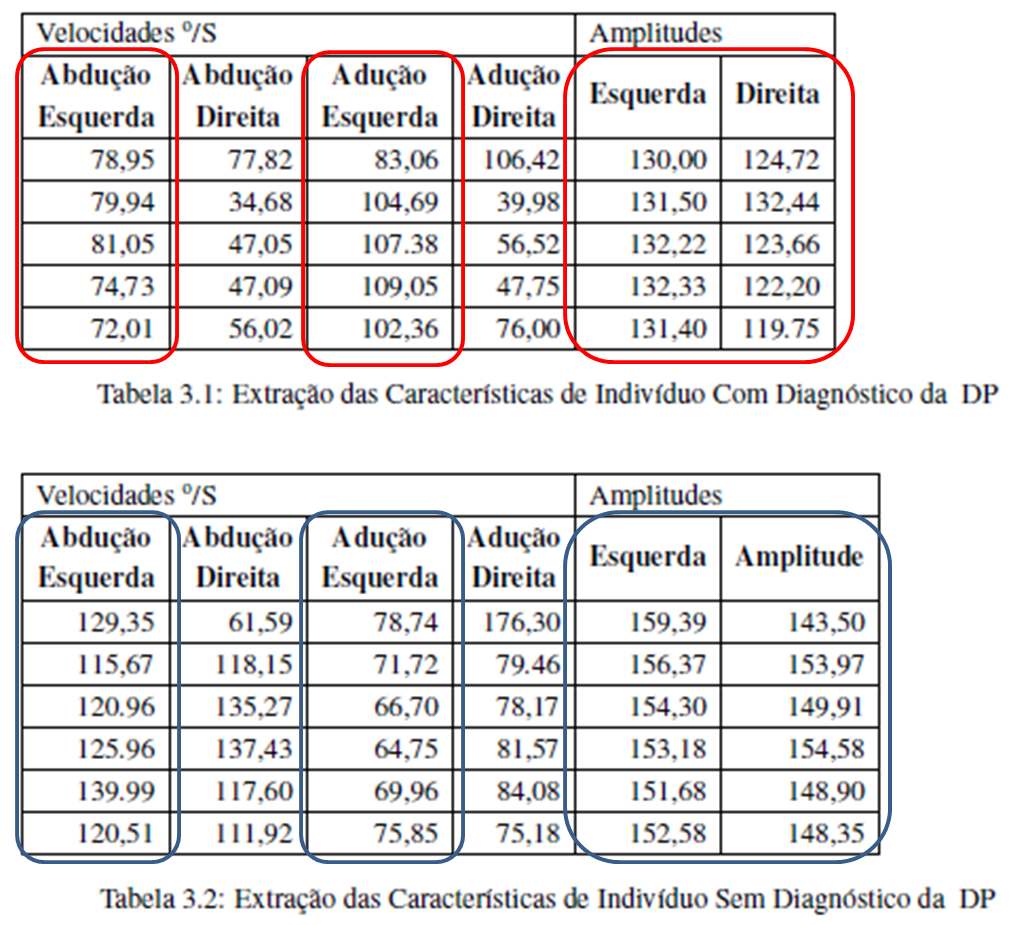
\includegraphics[height=2.6 in]{img/caracteristicas-tabela.png}
%   \end{block}
% \end{frame}

\section{Experimentos}
\subsection{Caso-Controle}
%\subsection{Estudo Analítico de Caso-Controle}
\begin{frame}{Estudo Analítico de Caso-Controle: Identificação da Bradicinesia} 
    \begin{block}{Objetivo da Pesquisa}

    
    Como melhor adquirir e quantificar sinais motores utilizando sensores de movimento para monitorar os sinais do Parkinson?

    \end{block}
		\begin{block}{Coleta de Dados}
			\begin{itemize}
				\item Protocolo de pesquisa submetido aprovado junto ao CEP da UFCG (\textbf{CAAE: 14408213.9.1001.5182})
				\item Coleta realizada nas instituições:
					\begin{enumerate}
						\item Hospital Universitário da UFAL
						\item Fundação Pestalozzi
						\item Clínica Fisioterapia do CESMAC
				\end{enumerate}				
			\end{itemize}
    \end{block}
\end{frame}

\begin{frame}{Amostra} 
    \begin{block}{}
			\begin{itemize}
				\item A técnica de amostragem utilizada para seleção, foi por conveniência, composta por:
				\begin{enumerate}
					\item 15 indivíduos portadores do Parkinson entre 51 e 65 anos (média de idade : 58 anos)
					\item 15 sem o diagnostico, como grupo controle entre 50 e 65 anos (média : 57 anos)
				\end{enumerate}
					\item No grupo de portadores do Parkinson, foram inclusos indivíduos até o Estágio 3 (Doença bilateral leve a moderada com alguma instabilidade postural e capacidade para viver independente), segundo a UPDRS
				\end{itemize}
    \end{block}
\end{frame}
 
\begin{frame}{Coleta dos Dados Utilizando o Jogo: \textit{Catch the Spheres}}
      \center 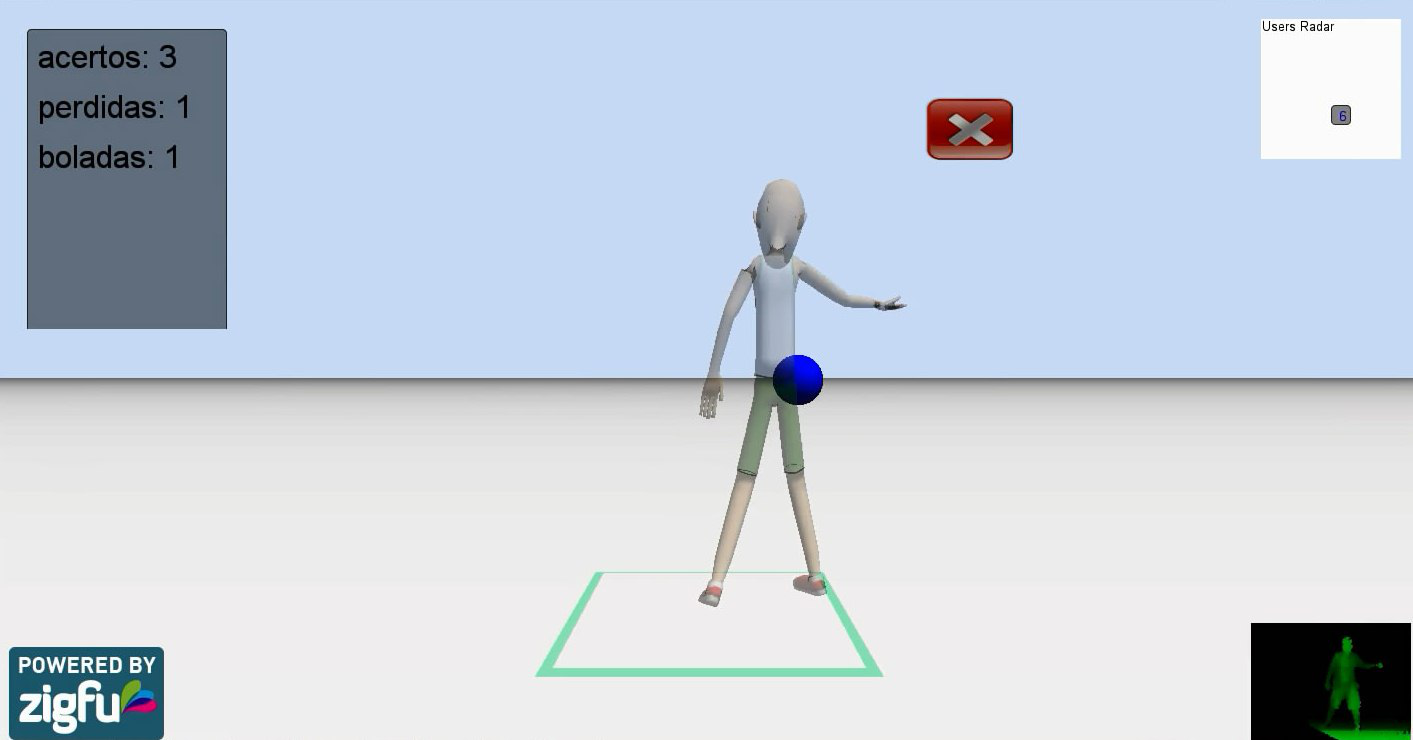
\includegraphics[height=2.2 in]{img/catch-the-spheres.png}
\end{frame}

\begin{frame}{Coleta de Dados}
  \begin{block}{}
  \center 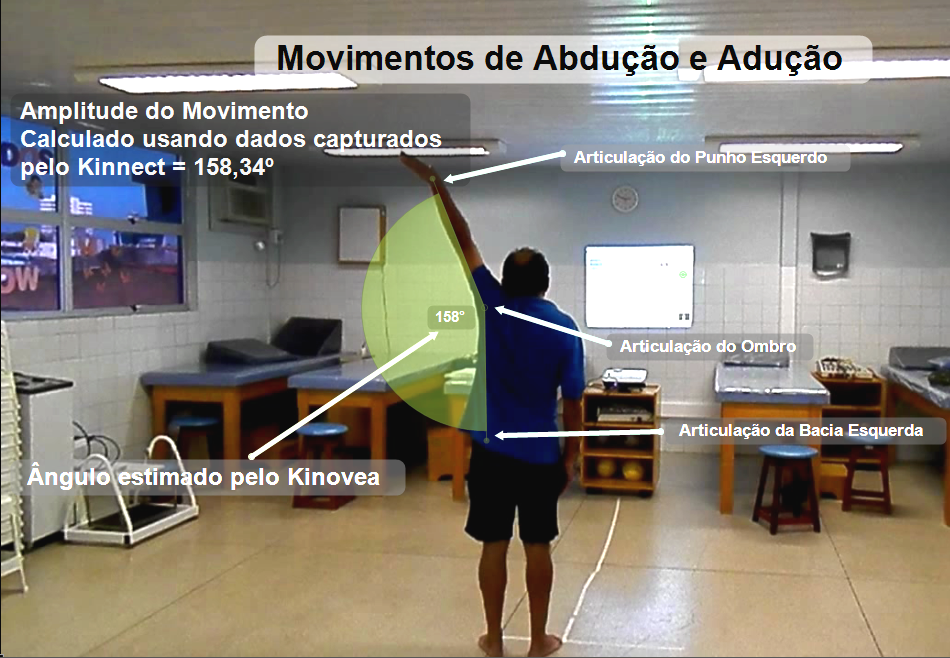
\includegraphics[height=2.4 in]{img/capturaducaokinnect.png} 
  \end{block}
\end{frame}



% \begin{frame}{Processo de Coleta de Dados}
%    \begin{block}{}   
%    \begin{columns}[c]
%      \begin{column}{0.5\linewidth}
% 				\begin{itemize}
% 					\item Voluntário se posiciona a 2m. do sensor de movimento
% 					\item Voluntário inicia o jogo
% 					\item Voluntário abduz e aduz o braço esquerdo, e depois o direito 10 vezes o mais amplo e rápido possível
% 					\item Voluntário fecha o jogo
% 				\end{itemize}
%      \end{column}
% 
%      \begin{column}{0.55\linewidth}
% 				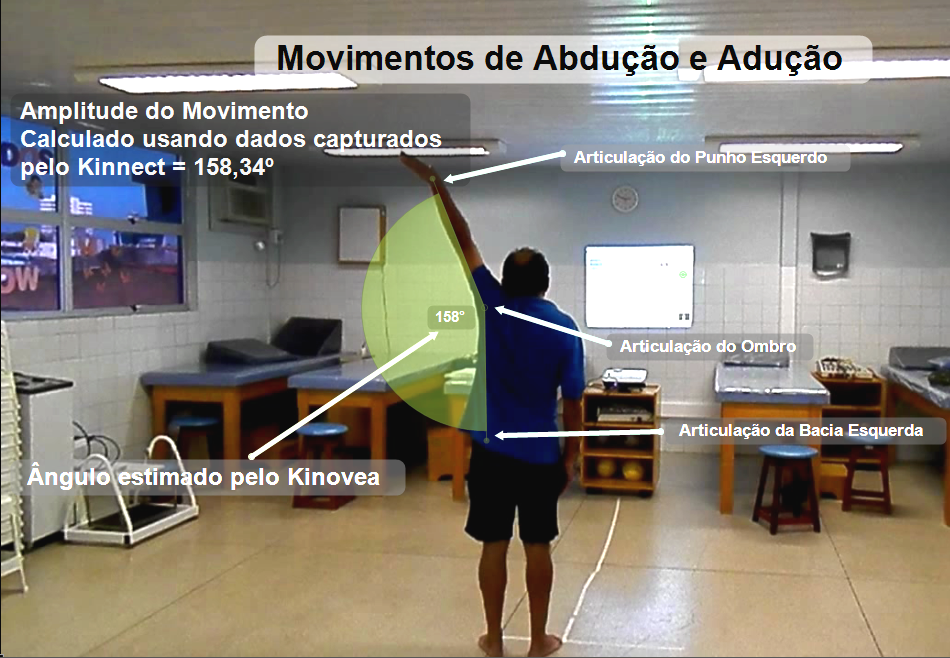
\includegraphics[width=5.5cm]{img/capturaducaokinnect.png}
%     \end{column}
% \end{columns}
% \end{block}
% \end{frame}
% 
% 
% 
% \begin{frame}{Processo de Coleta de Dados}
%   %\begin{block}{}
%       \center 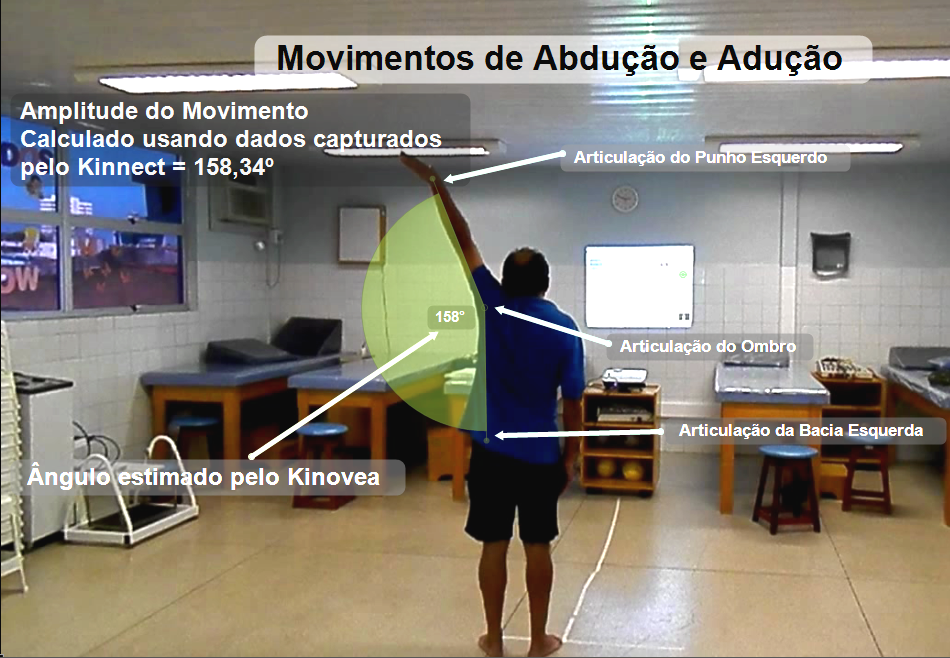
\includegraphics[height=2.6 in]{img/capturaducaokinnect.png}
% \end{frame}

% \begin{frame}{Características Extraídas do Movimento}
% 	\begin{block}{Descrição do vetor de características extraído da coleta de dados}
% 	\begin{table}[h]
% 	  \begin{tabular}{|l|l|}
% 	  \hline
% 	  {\bf Característica}  & {\bf Descrição}                                       \\ \hline
% 	  MaxAmpEsquerdo     & Amp. máxima do braço esquerdo. \\ \hline
% 	  MaxAmpDireito    & Amp. máxima do braço direito. \\ \hline
% 	  AngVelAbdEsquerdo  & Vel. ang. abdução do braço esquerdo. \\ \hline
% 	  AngVelAbdDireito & Vel. ang. da abdução do braço direito. \\ \hline
% 	  AngVelAdEsquerdo  & Vel. ang. da adução do braço esquerdo. \\ \hline
% 	  AngVelAdDireito & Vel. ang. de adução do braço direito. \\ \hline
% 	  \end{tabular}
% 	  \end{table}
% 
% 	
% % 		\begin{itemize}[<+->]
% % 			\item	Ciclo de movimento, normalizado e escalonado em 20 amostras;
% % 			\item	amplitude do movimento de abdução do braço esquerdo e direito;
% % 			\item	velocidade angular de abdução dos braços esquerdo e direito;
% % 			\item velocidade angular de adução do braço esquerdo e direito.
% % 		\end{itemize}
% 	\end{block}
% \end{frame}

\subsection{Classificação dos Dados}
\begin{frame}{Máquina de Vetor de Suporte (SVM)}
   \begin{block}{}
   
   \begin{columns}[c]
     \begin{column}{0.5\linewidth}
			 \begin{itemize}
			        \item Uma SVM busca encontrar vetores de suporte que consigam separa duas classes
			        
				%\item Uma SVM utiliza vetores de separação através de uma técnica de hiperplano de separação ótima

				\item Formalmente, essa classificador separa os dados por meio de um hiperplano através de uma função discriminante
			\end{itemize}
     \end{column}

     \begin{column}{0.5\linewidth}
				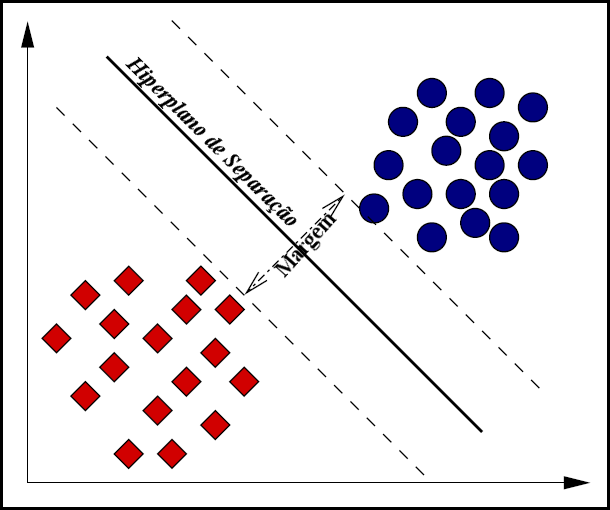
\includegraphics[width=4cm]{img/svmhyperplane.png}
    \end{column}
\end{columns}
\end{block}
\end{frame}

% \begin{frame}{Classificação dos Dados}
% 	\begin{block}{}
% 		\begin{itemize}
% 			\item	Com os dados coletados, realizou-se uma classificação usando SVM
% 			\item	Com os parâmetros de: $C = 2$ e $\gamma = 3$
% 		\end{itemize}
% 	\end{block}
% \end{frame}

%http://scikit-learn.org/stable/auto_examples/svm/plot_rbf_parameters.html
%http://www.eletrica.ufpr.br/ufpr2/professor/36/TE808/8-SVM-AM.pdf
%https://www.quora.com/What-are-C-and-gamma-with-regards-to-a-support-vector-machine

\begin{frame}{Optimização dos Parâmetros da SVM}
 \begin{block}{Aplicação do Método de \textit{Grid-Search}}
 Para identificar os melhores parâmetros da SVM, foi aplicado o método~\textit{Grid-Search} ~\cite{gridsearchsvm2010} usando validação cruzada \textit{Leave-One-Out}~\cite{kantardzic2011data}.   
 \end{block}
\end{frame}

%A standard SVM seeks to find a margin that separates all positive and negative examples


	
%C is the parameter for the soft margin cost function, which controls the influence of each individual support vector; this process involves trading error penalty for stability.

% Gamma is the free parameter of the Gaussian radial basis function.

%A small gamma means a Gaussian with a large variance so the influence of x_j is more, i.e. if x_j is a support vector, a small gamma implies the class of this support vector will have influence on deciding the class of the vector x_i even if the distance between them is large. If gamma is large, then variance is small implying the support vector does not have wide-spread influence. Technically speaking, large gamma leads to high bias and low variance models, and vice-versa.


%Intuitively, the gamma parameter defines how far the influence of a single training example reaches, with low values meaning ‘far’ and high values meaning ‘close’. The gamma parameters can be seen as the inverse of the radius of influence of samples selected by the model as support vectors.

%The C parameter trades off misclassification of training examples against simplicity of the decision surface. A low C makes the decision surface smooth, while a high C aims at classifying all training examples correctly by giving the model freedom to select more samples as support vectors.

\begin{frame}{Parâmetros da SVM}
   \begin{block}{Custo ($C$)}
   %$C$ (Custo) e $\gamma$ (Gamma) são os parâmetros de uma SVM não-linear RBF. \linebreak
   
   O $C$ é o parâmetro que controla a influência de individual de cada vetor de suporte no resultado da classificação. 
   
   %Um valor baixo do $C$ resulta numa superfície de decisão suave, enquanto que um alto valor para o $C$ dá mais liberdade para o modelo selecionar mais vetores de suporte.
   
   \end{block}
   
   \begin{block}{Gamma ($\gamma$)}
   O parâmetro $\gamma$ controla a flexibilidade da função de \textit{kernel}, valores pequenos de $\gamma$ permitem ao classificador ajustar todos os rótulos havendo risco de sobre ajustamento (\textit{overfitting}). 
   
   %Nesse caso o kernel da matriz se aproxima da matriz de identidade. Por outro lado, valores grandes de $\gamma$  reduzem o \textit{kernel} para uma função constante, tornando impossível o processo de aprendizagem do classificador.   
   \end{block}
\end{frame}

\begin{frame}{Optimização dos Parâmetros}
 \begin{block}{}
 O objetivo da optimização dos parâmetros é encontrar no espaço formado por ($\gamma$, $C$) pontos nos quais a acurácia do classificador seja a maior possível.
  
 Os valores dos parâmetros de pesquisa do \textit{grid-search} foram:
 \begin{itemize}
  \item $C$ = [$2^{-5}$, ... ,$2^2$]
  \item $\gamma$ = [$2^{-15}$, ... ,$2^3$]
 \end{itemize}

 Valores da Busca Detalhada:
  \begin{itemize}
   \item $C$ = [0.25, 0.5, ... ,2.5]
   \item $\gamma$ = [1, 2, ...,10]
  \end{itemize}
 \end{block}
 
 \begin{block}{Parâmetros Encontrados}
  Logo, usando o método \textit{grid-search}, encontramos os seguintes valores para os parâmetros: $C = 2$ e $\gamma = 3$
 \end{block}
\end{frame}

\begin{frame}{\textit{Grid-Search} - Acurácia da Classificação}
  \begin{block}{}
  \center  
  %\begin{block}{}
      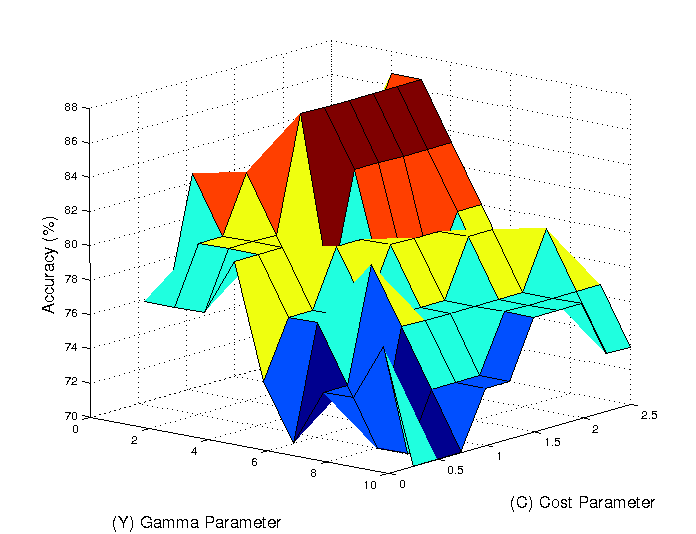
\includegraphics[scale=0.4]{./img/gridsearch.png}      
  \end{block}
\end{frame}

% \begin{frame}{\textit{Grid-Search} - \textit{FpRate}}
%    \begin{block}{}
%    \center
%   %\begin{block}{}
%       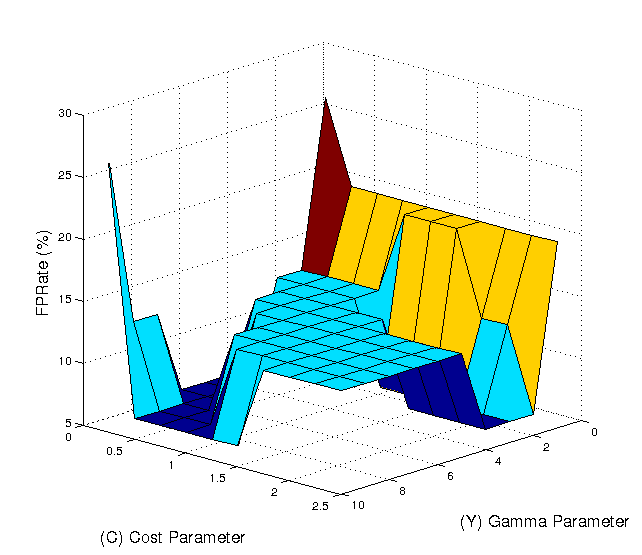
\includegraphics[scale=0.4]{./img/gridsearchfprate.png}
%    \end{block}
% \end{frame}

\begin{frame}{Matriz de Confusão do Estudo Analítico Caso-Controle Usando SVM}
	\begin{block}{}
\begin{table}[!htbp]
		\label{table:resultadomatrizconfusaosvm}
		\centering
		\begin{tabular}{l|c|c|}
		\cline{2-3}
		\multicolumn{1}{c}{}                         & \multicolumn{2}{|c|}{\textit{\textbf{Classe Preditiva}}} \\ \cline{2-3} 
																								 & \textbf{Parkinson}      & \textbf{Controle}         \\ \hline
		\multicolumn{1}{|l|}{\textbf{Parkinson}} & 12       & 3           \\ \hline
		\multicolumn{1}{|l|}{\textbf{Controle}}     & 1           & 14     \\ \hline
		\end{tabular}
\end{table}
	\end{block}
\end{frame}

\begin{frame}{Métricas da Classificação}
   %\begin{block}{}
				
		\begin{description}
			\item [\textit{TpRate}]: taxa de amostras positivas corretamente classificadas
			\item [\textit{FpRate}]: taxa de falso alarme obtido 
			\item [\textit{Accuracy}]:  taxa de amostras classificadas corretamente 
			\item [\textit{Precision}]: taxa de acerto de uma instância em determinada classe 
			\item [\textit{F-Measure}]: considera a média harmônica da taxa de \textit{precision} e do \textit{tp rate} 
		\end{description}

		
		\begin{table}[!htbp]
				\label{table:metricasmatrizconfusao}
				\centering
				\begin{tabular}{|l|r|}
				\hline
%				\multicolumn{2}{|l|}{\textbf{Métricas}} \\ \hline
				\textbf{TpRate}                    & 80,00$\%$\               \\ \hline
				\textbf{FpRate}                    & 6,67$\%$\                \\ \hline
				\textbf{Accuracy}                  & 86,67$\%$\                \\ \hline
				\textbf{Precision}                 & 92,31$\%$\                \\ \hline
				\textbf{F-Measure}                 & 85,71$\%$\                \\ \hline
				\end{tabular}
		\end{table}
% 		\begin{description}
% 			\item [\textit{TpRate}]: taxa de acerto obtido  ($ TpRate = TP/P $\ )
% 			\item [\textit{FpRate}]: taxa de falso alarme obtido : ($ FpRate = FP/N $\ ) 
% 			\item [\textit{Accuracy}]:  taxa de amostras positivas e negativas classificadas corretamente ($ Accuracy = (TP+TN)/(P+N) $\ )
% 			\item [\textit{Precision}]: taxa de acerto de uma instância em determinada classe ($ Precision =  TP/(TP +FP) $\ )
% 			\item [\textit{F-Measure}]: considera a média harmônica da taxa de \textit{precision} e do \textit{tp rate} ($ F-Measure = 2 * (Precision * TpRate)/(Precision + TpRate $\ )
% 		\end{description}

%	\end{block}
%     \begin{block}{}
%    \end{block}
\end{frame}


\begin{frame}{Outros Experimentos}
	\begin{block}{Uso de Jogo em \textit{Smartphone} Para Detecção de Tremor}
	\center 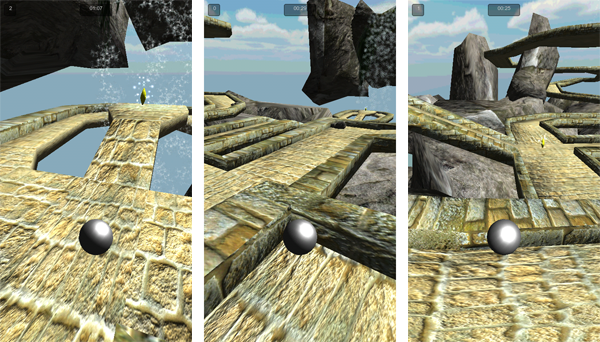
\includegraphics[height=1 in]{img/pinball_world.png}
	\end{block}
	\begin{block}{Insucesso na Quantificação do Tremor}
			\begin{itemize}
			\item Tremor do Parkinson é de repouso
			\item Indivíduos quando utilizavam o jogo reduziam drasticamente o sintoma
			\item Como os dados não seriam satisfatórios, logo a coleta tornou-se inviável
		\end{itemize}
	\end{block}
\end{frame}



\subsection{GQM}

\begin{frame}
  \begin{block}{ETAPA 3}
   Na perspectiva dos usuários, a abordagem de quantificar os sinais motores é considerada não-invasiva e aplicável à rotina diária?
  \end{block}
\end{frame}

% \begin{frame}{Análise GQM com Usuários} 
%     \begin{block}{Objetivo da Pesquisa}
%       Etapa 3 da Pesquisa: Na perspectiva dos usuários, a abordagem de quantificar os sinais motores é considerada não-invasiva e aplicável à rotina diária?
%     \end{block}
% % 		\begin{block}{Participantes}
% % 		Nessa etapa da pesquisa foram avaliados 30 sujeitos, dos seguintes locais: 
% % 			\begin{itemize}
% % 				\item Hospital Universitário da UFAL
% % 				\item Fundação Pestalozzi
% % 				\item Clínica de Fisioterapia do CESMAC
% % 			\end{itemize}
% %     \end{block}
% \end{frame} 


\begin{frame}{Questões da Pesquisa} 
    \begin{block}{}
			\begin{enumerate}
				\item O usuário poderia integrar a abordagem JOGUE-ME à sua rotina diária ?
				\item A segurança com a integridade física está de acordo com a faixa etária do usuário ?
			\end{enumerate}
    \end{block}
\end{frame}


%  \begin{table}[h]
%   \begin{tabular}{|p{10cm}|p{1.2cm}|p{1.2cm}|}
%   \hline
%   \textbf{Métrica} & \textbf{Sim} & \textbf{Não} \\ \hline
%   1.2: O jogo traz motivação ao usuário? & 91,67\% & 8,33\% \\ \hline
%   1.4: O usuário considera o jogo simples, sem muitas regras e de fácil entendimento? Ele pode ser aplicado em diferentes idades? & 91,67\% & 8,33\% \\ \hline
%   1.5: O usuário tem o costume de jogar esses jogos casuais em casa? & 41,67\% & 58,33\% \\ \hline
%   1.6: O usuário agregaria um jogo desse estilo em sua rotina diária? & 75\% & 25\% \\ \hline
%   2.1: Uma criança estaria segura jogando esse jogo, ao efetuar os movimentos dos braços? & 100\% & 0\% \\ \hline
%   2.2: Um adulto estaria seguro ao jogar esse jogo, ao efetuar os movimentos dos braços? & 100\% & 0\% \\ \hline
%   2.3: Um idoso estaria seguro ao jogar esse jogo, ao efetuar os movimentos dos braços? & 75\% & 25\% \\ \hline
%   \end{tabular}
%   \end{table}

% \begin{frame}{Métricas Avaliadas do \textit{GQM}} 
%   \begin{block}{Questão 1: Integração à Rotina Diária}
%     \begin{table}[h]
%   \begin{tabular}{|p{8cm}|p{1.2cm}|p{1.2cm}|}
%   \hline
%   \textbf{Métrica} & \textbf{Sim} & \textbf{Não} \\ \hline
%   1.2: O jogo traz motivação ao usuário? & 91,67\% & 8,33\% \\ \hline
%   1.4: O usuário considera o jogo simples, sem muitas regras e de fácil entendimento? Ele pode ser aplicado em diferentes idades? & 91,67\% & 8,33\% \\ \hline
%   1.5: O usuário tem o costume de jogar esses jogos casuais em casa? & 41,67\% & 58,33\% \\ \hline
%   1.6: O usuário agregaria um jogo desse estilo em sua rotina diária? & 75\% & 25\% \\ \hline
%   \end{tabular}
%   \end{table}
%   \end{block} 
% \end{frame}
% 
% \begin{frame}{Métricas Avaliadas do \textit{GQM}} 
%   \begin{block}{Questão 2: Segurança e Integridade Física}
%     \begin{table}[h]
%   \begin{tabular}{|p{8cm}|p{1.2cm}|p{1.2cm}|}
%   \hline
%   \textbf{Métrica} & \textbf{Sim} & \textbf{Não} \\ \hline
%   2.1: Uma criança estaria segura jogando esse jogo, ao efetuar os movimentos dos braços? & 100\% & 0\% \\ \hline
%   2.2: Um adulto estaria seguro ao jogar esse jogo, ao efetuar os movimentos dos braços? & 100\% & 0\% \\ \hline
%   2.3: Um idoso estaria seguro ao jogar esse jogo, ao efetuar os movimentos dos braços? & 75\% & 25\% \\ \hline
%   \end{tabular}
%   \end{table}
%   \end{block} 
% \end{frame}

\begin{frame}{Integrar a Abordagem à Rotina Diária} 
    %\begin{block}{}
			\center 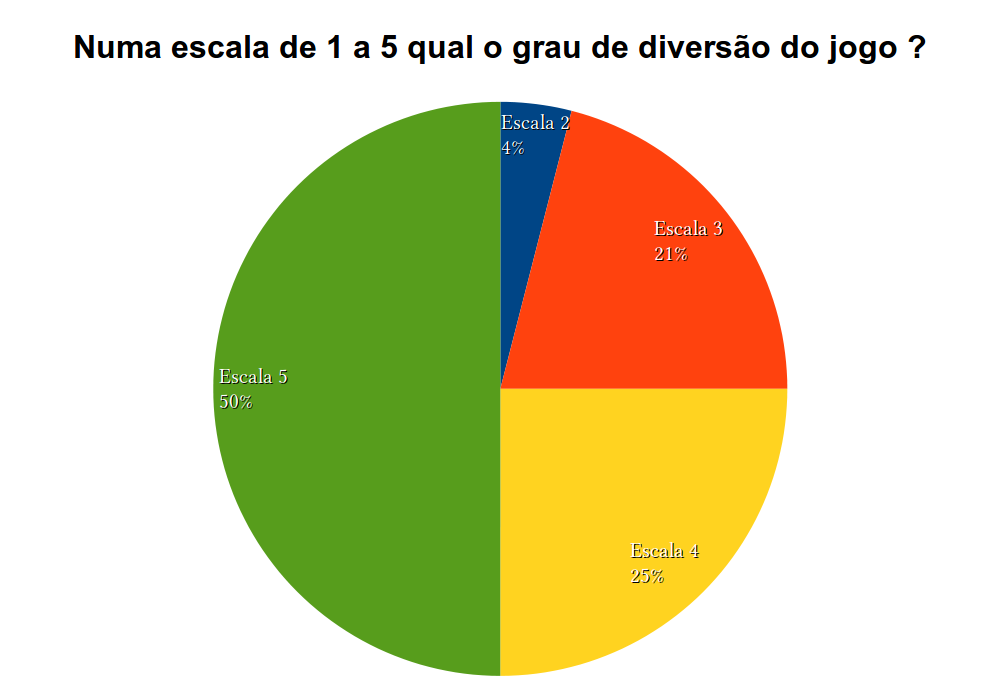
\includegraphics[height=2.8 in]{img/chartdiversao.png}
    %\end{block}
\end{frame}





\begin{frame}{Integrar a Abordagem à Rotina Diária} 
    %\begin{block}{Métrica 1.3: Integrar o Jogo À Rotina Diária}
			\center 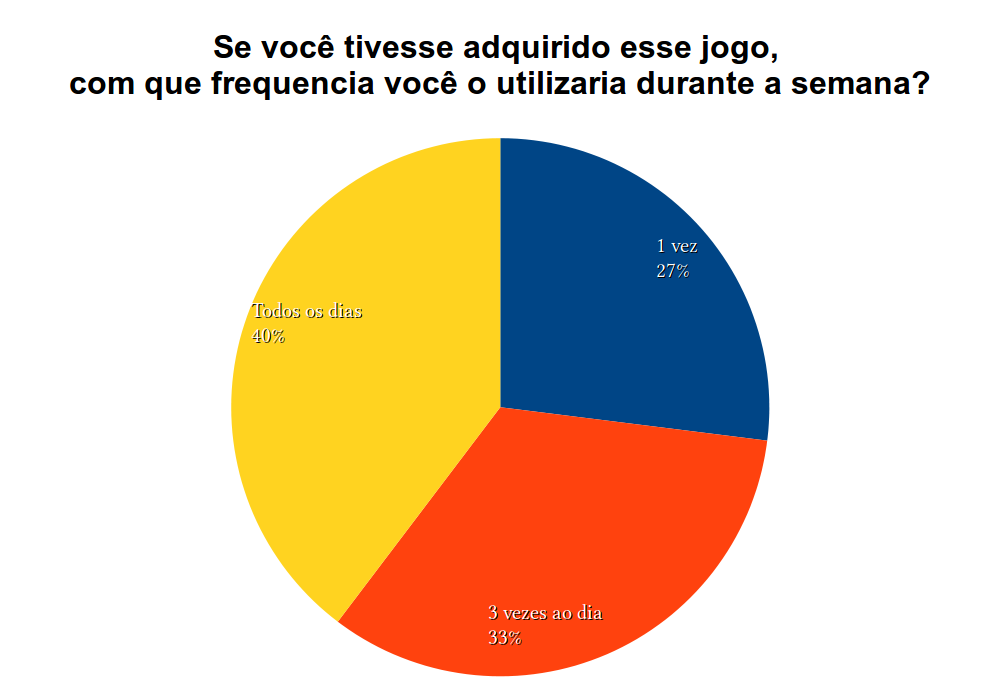
\includegraphics[height=2.8 in]{img/chartfrequencia.png}
    %\end{block}
\end{frame}

\begin{frame}{Integrar a Abordagem à Rotina Diária} 
    %\begin{block}{}
			\center 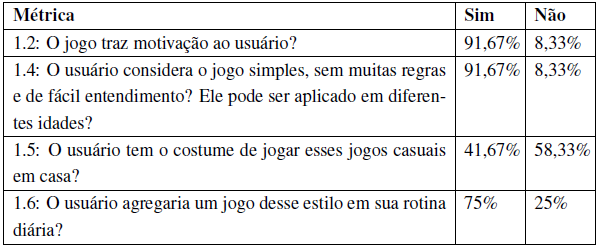
\includegraphics[height=1.4 in]{img/metricasq1.png}
    %\end{block}
\end{frame}

\begin{frame}{Segurança à Integridade Física} 
    %\begin{block}{Métrica 2.4: Faixa Etária do Jogo}
			\center 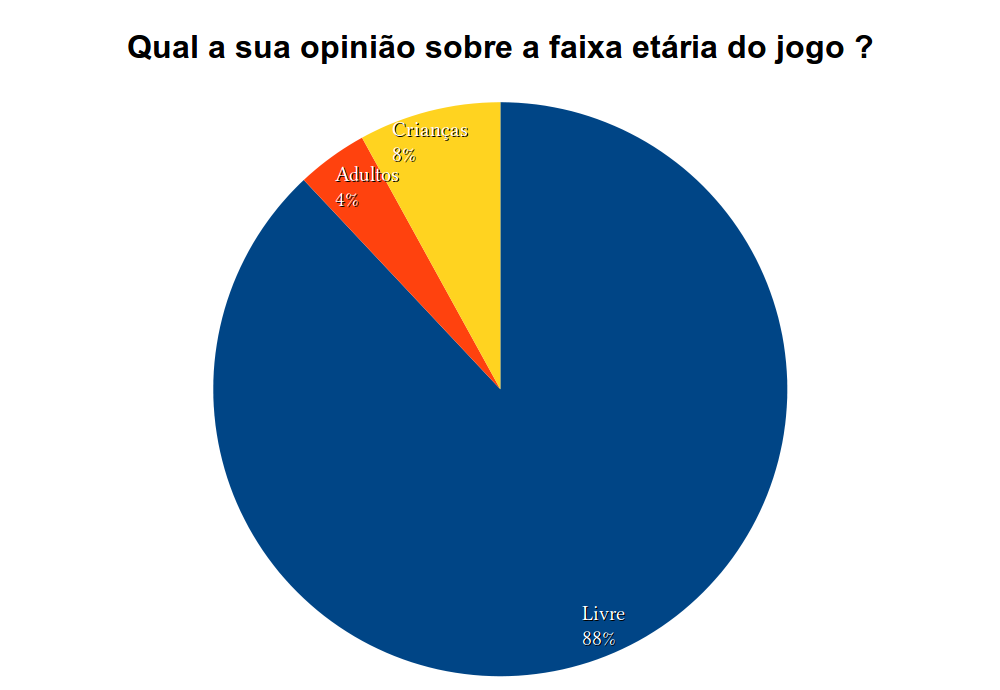
\includegraphics[height=2.8 in]{img/chartfaixaetaria.png}
    %\end{block}
\end{frame}

\begin{frame}{Segurança à Integridade Física} 
    \begin{block}{}
			\center 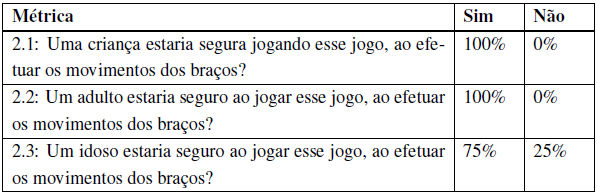
\includegraphics[height=1.4 in]{img/metricasq2.png}
    \end{block}
\end{frame}


\section{Conclusão e Trabalhos Futuros}
\subsection{}

\begin{frame}{Conclusão}
\begin{block}{}
Nos experimentos realizados, conseguimos demonstrar:
  \begin{itemize}
   \item A importância do acompanhamento dos sinais motores integrados à rotina diária do paciente
   \item A viabilidade do desenvolvimento de jogos para o monitoramento, pois, obtivemos uma taxa de acurácia de 86,67\% e falsos positivos de 6,67\%
   \item Um percentual de 83\% dos usuários integrariam a solução de monitoramento proposta em sua rotina diária
  \end{itemize}
\end{block}
\end{frame}

\begin{frame}{Trabalhos Futuros}
\begin{block}{}
A partir dos resultados apresentados nesta tese e extensão da mesma, alguns trabalhos futuros são propostos para contribuição científica:
  \begin{itemize}
   \item Coletar uma amostra maior de pacientes com Parkinson, e agrupá-los de acordo com o estágio da doença~\cite{goul05}
   \item Usar técnicas de multi-classificação de dados~\cite{multisvm2011} para identificar o progresso do Parkinson de acordo com as escalas de avaliação
   \item Avaliar o sinal da bradicinesia em diferentes momentos do dia, para verificar a eficácia do tratamento medicamentoso~\cite{protpar010}
  \end{itemize}
\end{block}
\end{frame}


%\subsection{Publicações}
\begin{frame}{Publicações}
\begin{block}{}
Foram publicados três artigos, em conferências internacionais, relacionados à tese: 
  \begin{itemize}
   \item \textit{Abstract}: \textbf{Monitoring Parkinson related Gait Disorders with Eigengaits}, \textit{XX World Congress on Parkinson's Disease and Related Disorders} (2013)%~\cite{lmmeigengaits2013}
   \item \textit{Full Paper}: \textbf{A Game-Based Approach to Monitor Parkinson’s Disease: The bradykinesia symptom classification}, \textit{International Symposium on Computer-Based Medical Systems} (CBMS 2016)%~\cite{lmmcbmsgame2016}
   \item \textit{Full Paper}: \textbf{A Gait Analysis Approach to Track Parkinson’s Disease Evolution Using Principal Component Analysis}, \textit{International Symposium on Computer-Based Medical Systems} (CBMS 2016)%~\cite{lmmcbmsgait2016}
  \end{itemize}
\end{block}
\end{frame}

%\subsection{Dúvidas}
\begin{frame}
  \begin{center}
  DÚVIDAS ?
  \end{center}
\end{frame}

\bibliographystyle{authordate2}
\bibliography{biblmmcor} % arquivos com as entradas bib.

\end{document}
	